Our first release of Travlendar+ includes all core functionalities of the application server and of the database server, as specified in the previous documents (more details in section \ref{sec:ApplAndDBServers} of this document), a set of initial functionalities in the Android application (more details in section \ref{sec:AndroidApp}) and does not include neither the web server implementation or the IOs app.
In the following schema we have highlighted the components of our general architecture (see also section 2.1 of DD) that are actually implemented and tested (components are encircled in green, the integration of the subsystems are colored in green). As stated before, in the following sections we will explain in details what exactly has been implemented.
\begin{figure}[H]
	\begin{center}
		\hspace*{-40pt}
		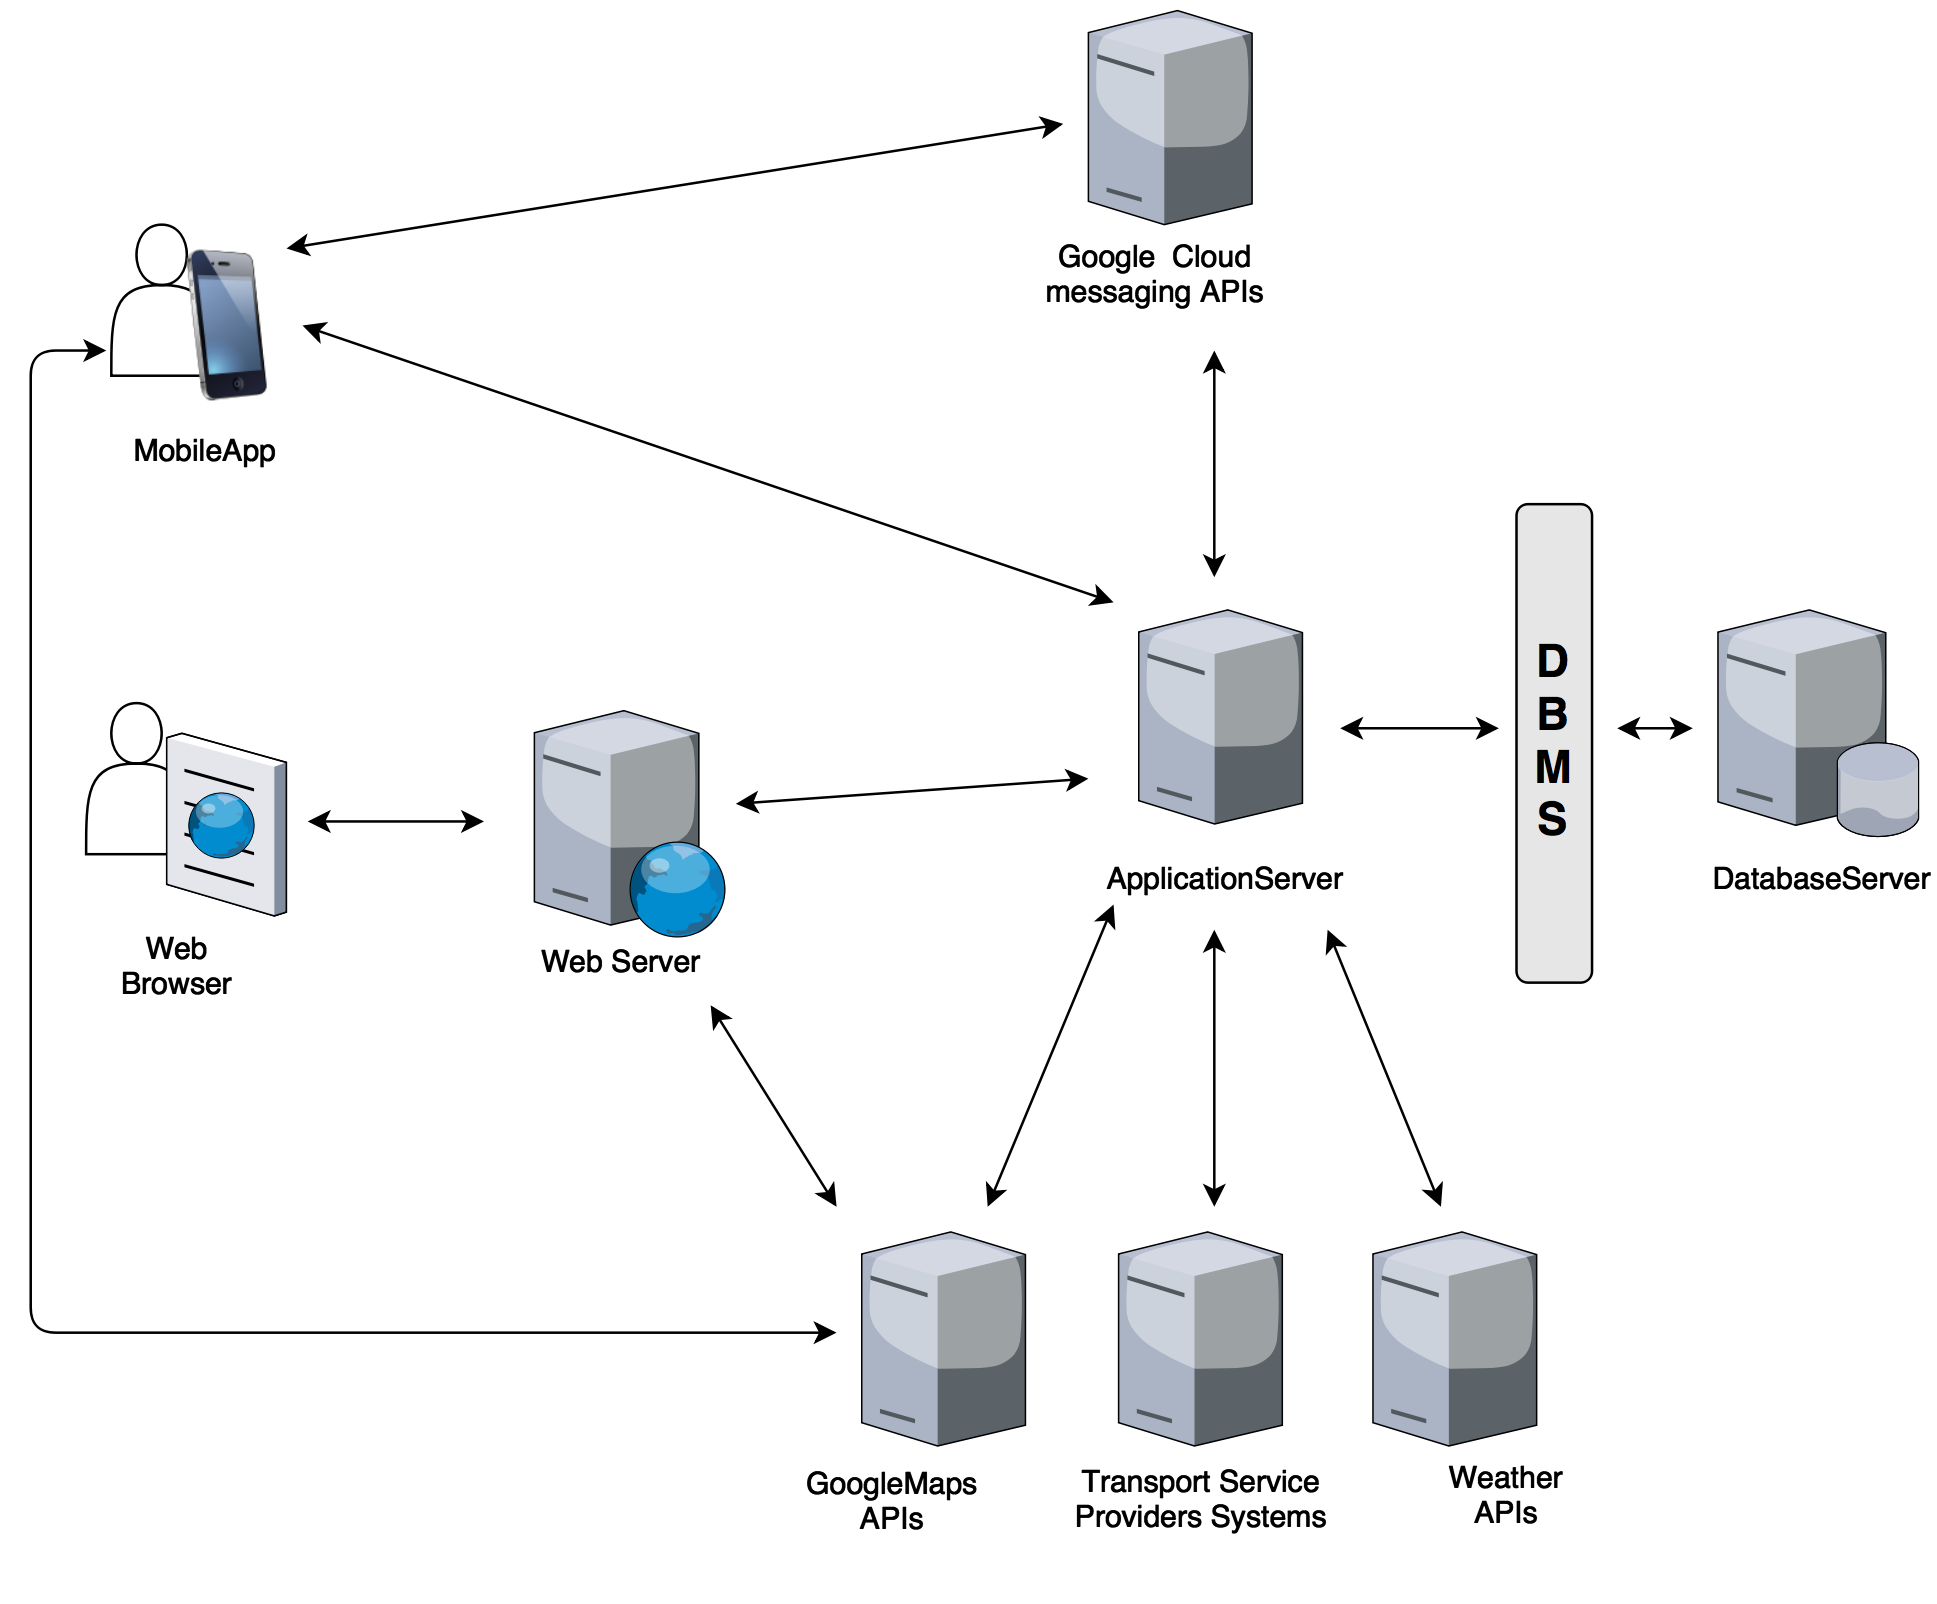
\includegraphics[scale=0.2]{GeneralArchitecture.png}
	\end{center}
\caption{General Architecture - Implemented subsystems}
\end{figure}

\newpage

\noindent Our software includes all the functionalities that:
\begin{itemize}
	\item Allow the users to have a calendar of events which can be either scheduled or non scheduled;
	\item Compute feasible travels which allow the users to reach their scheduled events in the allotted time;
	\item Allow the users to define their own preference profiles, which are to be applied to the travels proposed by our system;
	\item Allow the users to save their preferred locations into their profiles;
	\item Allow the users to define flexible breaks and to define periodical events;
	\item Allow the users to save their tickets and associate them to compatible travel components.
\end{itemize}
\noindent 
In this first release are not included the functionalities that:
\begin{itemize}
	\item Allow the users to buy new tickets within our application;
	\item Allow the users to locate the nearest sharing vehicles;
	\item Allow the system to take into account weather, forecast, strikes and traffic info and to notify the user if a path is no more feasible due to those issues.
\end{itemize} 
We have decided not to include them in our first release since we consider them as nice-to-have feature, but not mandatory for an initial release. They depend on other functionalities we have implemented and so they must come after those functionalities. We had then to choose how to allocate properly the limited amount of time given for the implementation phase and those functionalities would have required more time to be implemented. \\
Here we provide a list of use cases, taken from our RASD document (section 3.2.3) that are satisfied in this first release:
\begin{itemize}
	\item [UC1] Registration;
	\item [UC2] Login;
	\item [UC3] View calendar;
	\item [UC4] Create event;
	\item [UC5] Create personalized event profiles;
	\item [UC6] Define flexible breaks;
	\item [UC7] Arrange trips - Only with ticket inserted by the user;
	\item [UC9] Add ticket possessed;
	\item [UC10] Obtain feasible travel paths - Without the alternatives paths;
	\item [UC11] Choose between overlapping events;
	\item [UC12] Edit event - Only in Application server, not yet available on Android app; 
	\item [UC13] Delete event;
	\item [UC14] Edit personalized event profiles;
	\item [UC15] Delete personalized event profiles.
\end{itemize}

\section{Application Server and Database Server}
\label{sec:ApplAndDBServers}
In this section we specify which requirements are actually implemented in our ApplicationServer subsystem, examining every sub-component, and stating which requirements are implemented in this first release of Travlendar+. We also state the motivations for including them and excluding others (see also chapter 5 of DD - requirement traceability).
\begin{figure}[H]
	\begin{center}
		\hspace*{-60pt}
		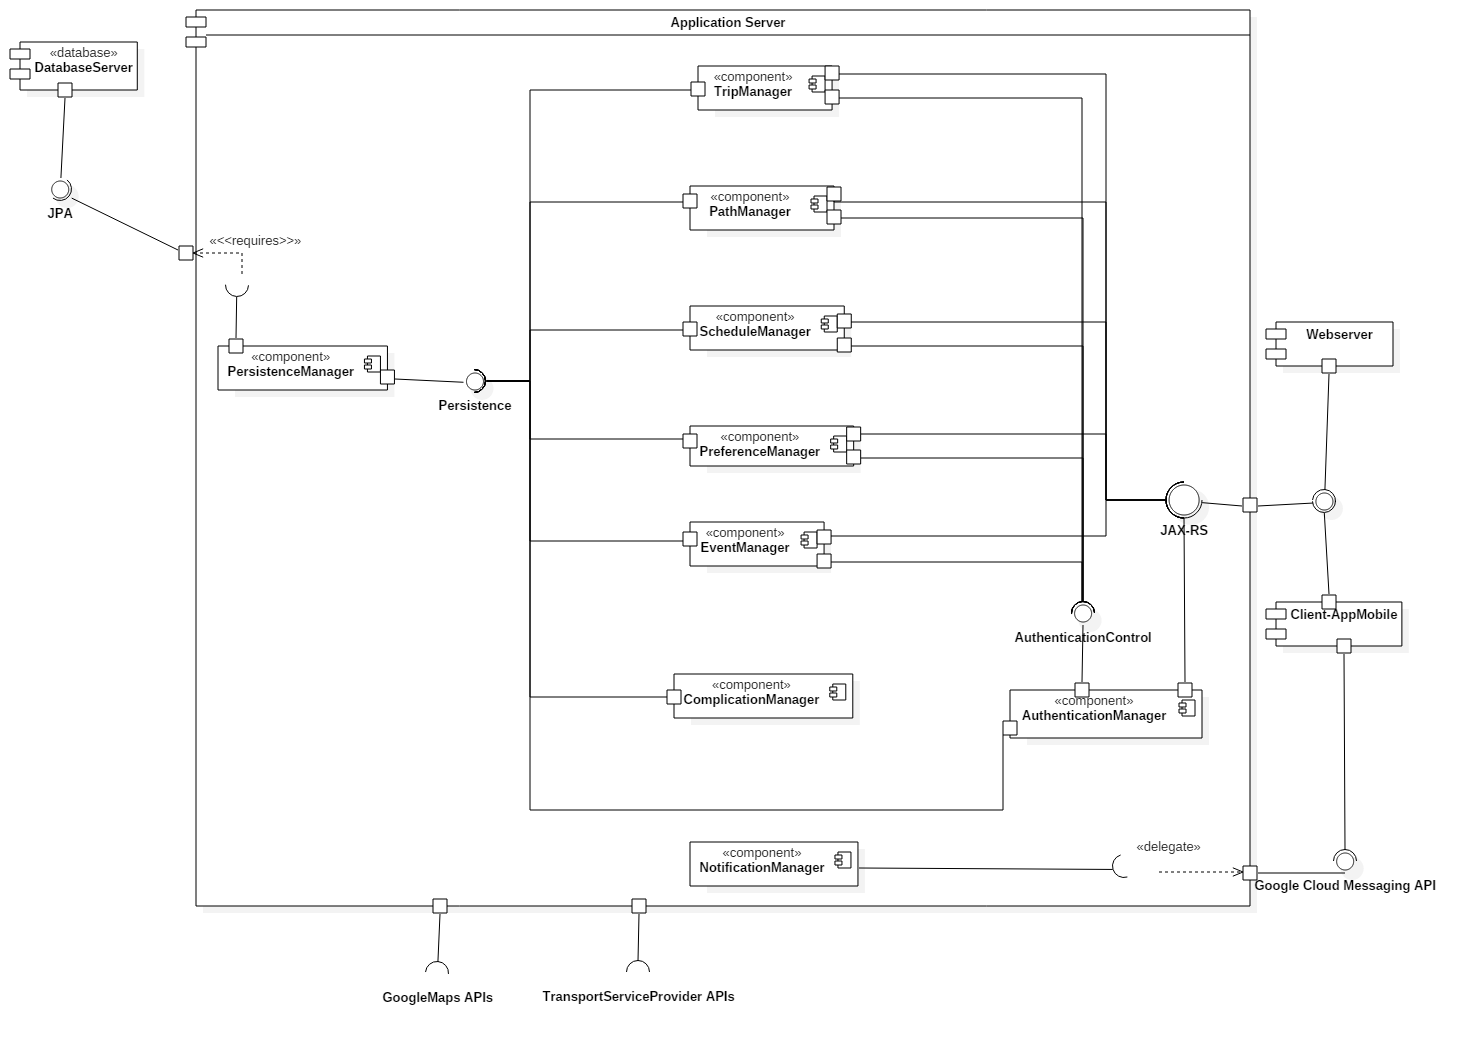
\includegraphics[scale=0.4]{ApplicationServer.png}
	\end{center}
\caption{The implemented components of the Application Server}
\end{figure}

\subsection{Authentication Manager}
All the requirements related to the authentication manager are fulfilled in this first release: the user can register himself into the system, log in from any device he prefers (but only one at the time), modify his account's info, delete his account and request a new password. \\
As specified in the previous documents, these are the requirements met by this manager:
\begin{itemize}
	\item \textbf{[R1]} the system checks if the e-mail inserted is real;
	\item \textbf{[R2]} a user cannot sign up with the same e-mail twice;
	\item \textbf{[R3]} the e-mail and password inserted must be correct;
	\item \textbf{[R4]} incorrect credentials prevent the user from logging in;
	\item \textbf{[R38]} a user must be logged.
\end{itemize}

\subsection{Event Manager}
Event manager handles insertion, deletion and modification of both events and break events into the user's calendar.
It interacts with both path and schedule manager in order to provide feasible paths to the events and to decide whether they can be scheduled or not.
In the application server also the propagation of periodical events through the time is handled properly. \\
In our system is not yet handled the possibility to modify and delete with one operation all the periodic events generated from one single event, due to time-related issues.
In our system is not yet handled the possibility to define events without an ending time since we do not consider this feature essential, but just an optional and not so necessary feature. \\
As specified in the previous documents, these are the requirements met by this manager:
\begin{itemize}
	\item \textbf{[R5]} a user must specify all mandatory fields to add the new event;
	\item \textbf{[R6]} the system reserves the specified time-slot for the event;
	\item \textbf{[R7]} the system warns the user if the inserted event overlaps with an already existing one;
	\item \textbf{[R29]} the system allows the user to specify a flexible interval and a minimum amount of time to schedule a break.
\end{itemize}
And these are the requirements not yet implemented in this manager:
\begin{itemize}
	\item \textbf{[R8]} if the ending time of an event is not specified, the systems considers as ending time the hour of departure for the successive event;
	\item \textbf{[R9]} when an event is inserted after an event without a specified ending time, the ending time  of the first event is anticipated as stated in [R8].
\end{itemize}

\subsection{Preference Manager}
All the requirements related to the preference manager are fulfilled.
This module offers all the functionalities needed to insert, modify and delete the user's event profiles and the user's preferred locations. It is also able to apply the user's preferences to the feasible travels computed by our system. \\
As specified in the previous documents, these are the requirements met by this manager:
\begin{itemize}
	\item \textbf{[R12]} the system does not consider paths that violate constraints on travel means defined by the user;
	\item \textbf{[R13]} the system checks user preferences to decide which feasible travel path is the best;
	\item \textbf{[R15]} appropriate travel means must be suggested according to the type of event that they are related to;
	\item  \textbf{[R23]} the system requires minimum and maximum length allowed for a path to impose a constraint on a travel mean;
	\item \textbf{[R24]} the system requires an interval of time allowed to impose a constraint on a travel mean;
	\item \textbf{[R25]} the system does not consider solutions that violate constraints;
	\item \textbf{[R26]} the system allows the user to specify one or more travel means that cannot be used;
	\item \textbf{[R27]} the system does not consider solutions that include deactivated travel means.
\end{itemize}

\subsection{Path Manager}
This module manages the feasible travels computation, after the insertion or the modification of an event. It interacts with the \textit{PreferenceManager} in order to obtain the information needed to guarantee that the user preferences are respected in every proposed path.\\
The functionalities that allow to change a selected path, choosing between a set of feasible alternatives, to obtain info that allow to draw a feasible path on a map and to obtain also options that include sharing vehicles are not yet available; we've chosen not to include them due to time-related issues and because they would have been nice-to-have features but not essential for an initial release. \\
As specified in the previous documents, these are the requirements met by this manager:
\begin{itemize}
	\item \textbf{[R10]} every travel path proposed must be feasible in the available time (the interval between two consecutive events);
	\item \textbf{[R11]} if the travel involves two or more travel means, the starting location of the first proposed travel path and the ending location of the last proposed travel path must coincide respectively with the starting location and the ending location of the whole planned travel;
	\item \textbf{[R12]} the system does not consider paths that violate constraints on travel means defined by the user;
	\item \textbf{[R13]} the system checks user preferences to decide which feasible travel path is the best;
	\item \textbf{[R15]} appropriate travel means must be suggested according to the type of event that they are related to;
	\item \textbf{[R25]} the system does not consider solutions that violate constraints;
	\item \textbf{[R27]} the system does not consider solutions that include deactivated travel means;
	\item \textbf{[R35]} the system provides information about time of departure and arrival of the proposed travels.
\end{itemize}
And these are the requirements not yet implemented in this manager:
\begin{itemize}
	\item \textbf{[R18]} the system must show to the user all possibilities to reach a location in according with the requirements of [G4];
	\item \textbf{[R19]} alternative feasible travel paths must not generate overlappings with other events of the schedule;
	\item \textbf{[R28]} for each travel path, the system estimates its carbon footprint produced;
	\item \textbf{[R37]} the system provides information about travel time with shared vehicles.
\end{itemize}

\subsection{Schedule Manager}
This module is able to check if an event overlaps with other events and to guarantee that the flexible breaks are respected. It also checks that the user's travels do not overlap with other events. When an event overlaps with another one, the schedule manager puts it in a separate list of non scheduled events and it manages the user's requests of rescheduling those events. \\
As specified in the previous sections, events without an ending time and alternative travels are not yet implemented into our system since, due to time-related issues, we've decided to exclude them from our first release of Travlendar+. \\
As specified in the previous documents, these are the requirements met by this manager:
\begin{itemize}
	\item \textbf{[R6]} the system reserves the specified time-slot for the event;
	\item \textbf{[R7]} the system warns the user if the inserted event overlaps with an already existing one;
	\item \textbf{[R14]} the system warns the user if it is not possible to arrive at an event location before its starting time;
	\item \textbf{[R20]} the combination of the travel paths proposed for the day must be feasible in the allotted time;
	\item \textbf{[R21]} if there are multiple events at the same time the system will propose in the schedule only the first event added;
	\item \textbf{[R22]} if the user forces into the schedule an event that overlaps with events already present in the schedule, these are removed from the schedule;
	\item \textbf{[R30]} if there is enough time for a break, the system reserves it within the specified flexible interval;
	\item \textbf{[R31]} if there is not enough time into the flexible interval specified, a warning is thrown.
\end{itemize}

And these are the requirements not yet implemented in this manager:
\begin{itemize}
	\item \textbf{[R8]} if the ending time of an event is not specified, the systems considers as ending time the hour of departure for the successive event;
	\item \textbf{[R9]} when an event is inserted after an event without a specified ending time, the ending time  of the first event is anticipated as stated in [R8];
	\item \textbf{[R19]} alternative feasible travel paths must not generate overlappings with other events of the schedule.
\end{itemize}

\subsection{Trip Manager}
Trip manager is the last module we have implemented and offers only the functionalities that allow the user to save and visualize his tickets and to associate them to travel components for which they are applicable. \\
This module does not yet provide functionalities that allow the user to buy public transportation tickets and to locate the nearest sharing vehicles, since they would have required the integration of other external APIs and we have decided to allocate our time in other functionalities that we consider more important than these ones. \\
As specified in the previous documents, these are the requirements met by this manager:
\begin{itemize}
	\item \textbf{[R32]} the system allows the user to specify all the ticket he already owns;
	\item \textbf{[R33]} the system shows to the user if he already holds a ticket for a proposed travel;
\end{itemize}
And these are the requirements not yet implemented in this manager:
\begin{itemize}
	\item \textbf{[R34]} the system allows the user to buy public transportation tickets according to proposed travels;
	\item \textbf{[R36]} the system shows to the user where sharing vehicles are located.
\end{itemize}
\newpage
\subsection{Complication manager and Notification Manager}
Both Complication and Notification manager are not implemented in this first release of Travlendar+, since we have considered their functionalities not essential for the first release of our system and since we had to make a choice due to limited implementation time. 

\section{Android App}
\label{sec:AndroidApp}
In this section we specify which requirements are actually implemented in our first release of Travlendar+'s Android app.
Our Android application implements all the functionalities that are offered by our application server (for more details please refer to the previous sections) except: 
\begin{itemize}
	\item periodical events insertion;
	\item modifications of already inserted events and break events, only their deletion is available;
	\item modifications of already inserted tickets, only their deletion is available;
	\item user profile deletion and modification.
\end{itemize}
Furthermore the map interface does not work yet.\\
\noindent 
These are the requirements met by our Android application:
\begin{itemize}
	\item \textbf{[R1]} the system checks if the e-mail inserted is real;
	\item \textbf{[R2]} a user cannot sign up with the same e-mail twice;
	\item \textbf{[R3]} the e-mail and password inserted must be correct;
	\item \textbf{[R4]} incorrect credentials prevent the user from logging in; 
	\item \textbf{[R5]} a user must specify all mandatory fields to add the new event;
	\item \textbf{[R6]} the system reserves the specified time-slot for the event;
	\item \textbf{[R7]} the system warns the user if the inserted event overlaps with an already existing one;
	\item \textbf{[R10]} every travel path proposed must be feasible in the available time (the interval between two consecutive events);
	\item \textbf{[R11]} if the travel involves two or more travel means, the starting location of the first proposed travel path and the ending location of the last proposed travel path must coincide respectively with the starting location and the ending location of the whole planned travel;
	\item \textbf{[R12]} the system does not consider paths that violate constraints on travel means defined by the user;
	\item \textbf{[R13]} the system checks user preferences to decide which feasible travel path is the best;
	\item \textbf{[R14]} the system warns the user if it is not possible to arrive at an event location before its starting time;
	\item \textbf{[R15]} appropriate travel means must be suggested according to the type of event that they are related to; 
	\item \textbf{[R20]} the combination of the travel paths proposed for the day must be feasible in the allotted time;
	\item \textbf{[R21]} if there are multiple events at the same time the system will propose in the schedule only the first event added;
	\item \textbf{[R22]} if the user forces into the schedule an event that overlaps with events already present in the schedule, these are removed from the schedule;
	\item \textbf{[R23]} the system requires minimum and maximum length allowed for a path to impose a constraint on a travel mean;
	\item \textbf{[R24]} the system requires an interval of time allowed to impose a constraint on a travel mean;
	\item \textbf{[R25]} the system does not consider solutions that violate constraints;
	\item \textbf{[R26]} the system allows the user to specify one or more travel means that cannot be used;
	\item \textbf{[R27]} the system does not consider solutions that include deactivated travel means; 
	\item \textbf{[R29]} the system allows the user to specify a flexible interval and a minimum amount of time to schedule a break;
	\item \textbf{[R30]} if there is enough time for a break, the system reserves it within the specified flexible interval;
	\item \textbf{[R31]} if there is not enough time into the flexible interval specified, a warning is thrown;
	\item \textbf{[R32]} the system allows the user to specify all the ticket he already owns;
	\item \textbf{[R33]} the system shows to the user if he already holds a ticket for a proposed travel;
	\item \textbf{[R35]} the system provides information about time of departure and arrival of the proposed travels;
	\item \textbf{[R38]} a user must be logged. 
\end{itemize}

And these are the requirements not yet implemented in our Android application:
\begin{itemize}
	\item \textbf{[R8]} if the ending time of an event is not specified, the systems considers as ending time the hour of departure for the successive event;
	\item \textbf{[R9]} when an event is inserted after an event without a specified ending time, the ending time  of the first event is anticipated as stated in [R8];
	\item \textbf{[R16]} if a strike occurs, the system will not consider travel means involved in it;
	\item \textbf{[R17]} if the weather forecasts rain or other adverse conditions, the system will not consider paths involving the bicycle;
	\item \textbf{ [R18]} the system must show to the user all possibilities to reach a location in according with the requirements of [G4];
	\item \textbf{[R19]} alternative feasible travel paths must not generate overlappings with other events of the schedule;
	\item \textbf{[R28]} for each travel path, the system estimates its carbon footprint produced;
	\item \textbf{[R34]} the system allows the user to buy public transportation tickets according to proposed travels;
	\item \textbf{[R36]} the system shows to the user where sharing vehicles are located;
	\item \textbf{[R37]} the system provides information about travel time with shared vehicles;
\end{itemize}
